\documentclass{beamer}
\usepackage[utf8]{inputenc}
\usepackage[ngerman]{babel}
\usepackage{lastpage}

\input{flat-blue-theme.inc}

\author[Hauke Stieler]{Hauke Stieler\\\href{mailto:4stieler@informatik.uni-hamburg.de}{4stieler@inf}}
\title{Wie man (nicht) zur Venus reist}
\date{\today}

\begin{document}
	\maketitle\newpage
	\tableofcontents[hidesubsections]\newpage
	\begin{frame}
		\begin{figure}[ht]
			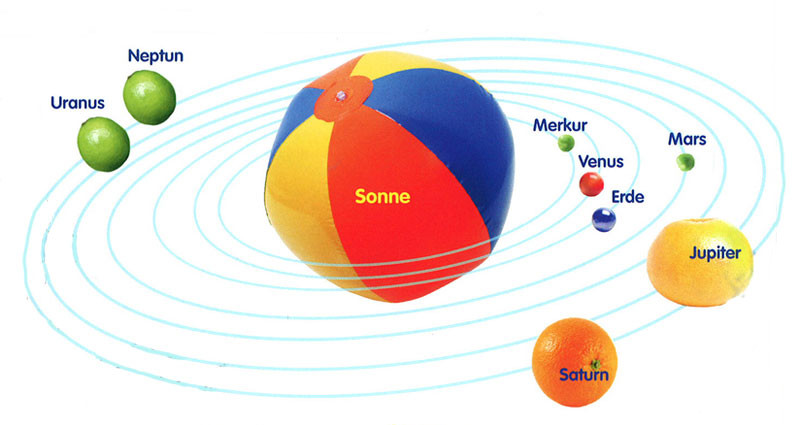
\includegraphics[scale=0.4]{./images/sonnensystem}
		\end{figure}
		{\tiny * Darstellung ggf. nicht Maßstabsgetreu}
	\end{frame}
	\begin{frame}
		\begin{figure}[ht]
%			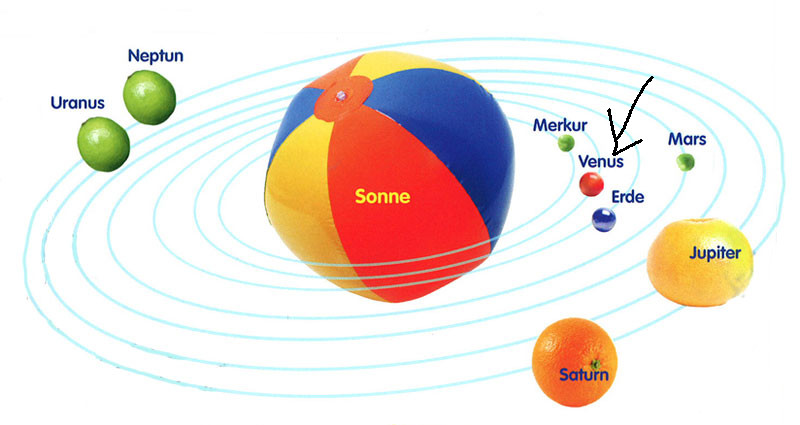
\includegraphics[scale=0.4]{./images/sonnensystem2}
			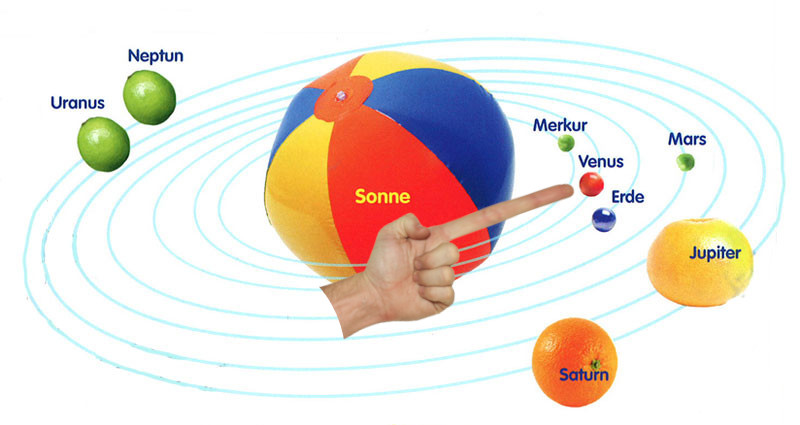
\includegraphics[scale=0.4]{./images/sonnensystem2finger}
		\end{figure}
		{\tiny * Darstellung ggf. nicht Maßstabsgetreu}
	\end{frame}
	\section{Venera 1 bis 8}
	\subsection{Venera 1}
	\begin{frame}
		\begin{columns}
			\begin{column}{0.5\textwidth}
				\begin{itemize}
					\item 1961
					\item Kontaktverlust nach 7 Tagen
					\item Flog 100.000km an Venus vorbei
				\end{itemize}
			\end{column}
			\begin{column}{0.4\textwidth}
				\begin{figure}[ht]
					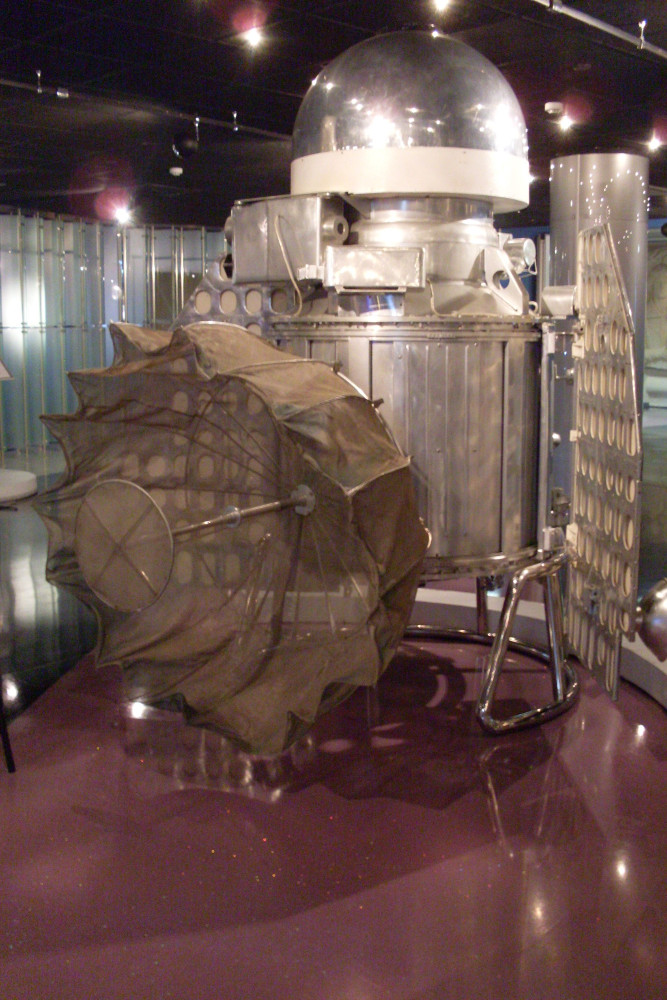
\includegraphics[scale=0.21]{./images/venera_1}
				\end{figure}
			\end{column}
		\end{columns}
	\end{frame}
	\subsection{Venera 2}
	\begin{frame}
		\begin{columns}
			\begin{column}{0.5\textwidth}
				\begin{itemize}
					\item 1965
					\item Kontaktverlust kurz vor Vorbeiflug
				\end{itemize}
			\end{column}
			\begin{column}{0.4\textwidth}
				\begin{figure}[ht]
					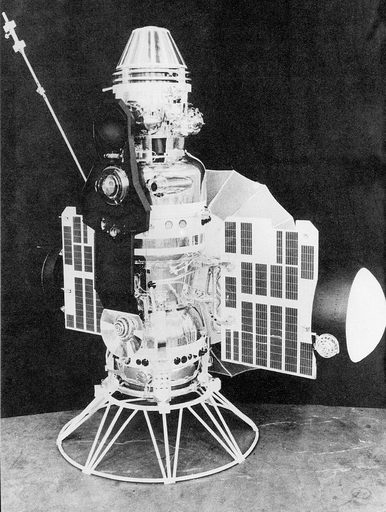
\includegraphics[scale=0.3]{./images/venera_2}
				\end{figure}
			\end{column}
		\end{columns}
	\end{frame}
	\subsection{Venera 3}
	\begin{frame}
		\begin{columns}
			\begin{column}{0.5\textwidth}
				\begin{itemize}
					\item 1965
					\item Auch Kontaktverlust kurz vor Vorbeiflug
					\item Klingte Landesone ab
					\item Sonde verglühte
				\end{itemize}
			\end{column}
			\begin{column}{0.4\textwidth}
				\begin{figure}[ht]
					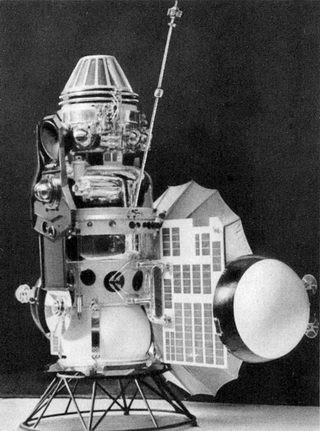
\includegraphics[scale=0.4]{./images/venera_3}
				\end{figure}
			\end{column}
		\end{columns}
	\end{frame}
	\subsection{Venera 4}
	\begin{frame}
		\begin{columns}
			\begin{column}{0.5\textwidth}
				\begin{itemize}
					\item 1967
					\item Klinke Landesonde ab
					\item Fiel nach 96 Minuten aus (Batterien alle)
					\item Oberfläche nicht erreicht
					\begin{itemize}
						\item Atmosphärendruck zu hoch
						\item Landung dauerte zu lange
					\end{itemize}
					\item In 25km Höhe 270$^\circ$C und 22 bar
				\end{itemize}
			\end{column}
			\begin{column}{0.4\textwidth}
				\begin{figure}[ht]
					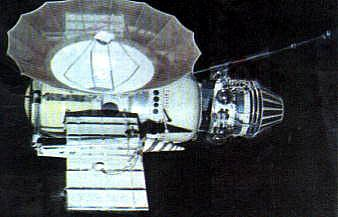
\includegraphics[scale=0.4]{./images/venera_4}
				\end{figure}
			\end{column}
		\end{columns}
	\end{frame}
	\subsection{Venera 5}
	\begin{frame}
		\begin{columns}
			\begin{column}{0.5\textwidth}
				\begin{itemize}
					\item 1969
					\item Klinke Landesonde ab
					\item Versagte nach 53 Minuten (schmolz und wurde zerdrückt)
					\item In 24-26km Höhe 320$^\circ$C und 26 bar
				\end{itemize}
			\end{column}
			\begin{column}{0.4\textwidth}
				\begin{figure}[ht]
					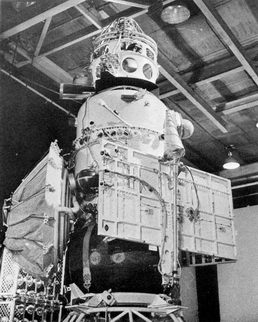
\includegraphics[scale=0.4]{./images/venera_5}
				\end{figure}
			\end{column}
		\end{columns}
	\end{frame}
	\subsection{Venera 6}
	\begin{frame}
		\begin{columns}
			\begin{column}{0.5\textwidth}
				\begin{itemize}
					\item 1969
					\item Baugleich mit Venera 5
					\item Klinke Landesonde ab
					\item Versagte nach 53 Minuten (schmolz und wurde zerdrückt)
				\end{itemize}
			\end{column}
			\begin{column}{0.4\textwidth}
				\begin{figure}[ht]
					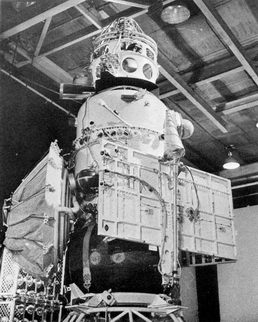
\includegraphics[scale=0.4]{./images/venera_5}
				\end{figure}
			\end{column}
		\end{columns}
	\end{frame}
	\subsection{Venera 7}
	\begin{frame}
		\begin{columns}
			\begin{column}{0.5\textwidth}
				\begin{itemize}
					\item 1970
					\item Sonde Landete tatsächlich :o
					\item Kippte beim landen um -.-
					\item Auf Oberfläche waren 475$^\circ$C und 92bar
					\item Schmolz nach 21 Minuten
				\end{itemize}
			\end{column}
			\begin{column}{0.4\textwidth}
				\begin{figure}[ht]
					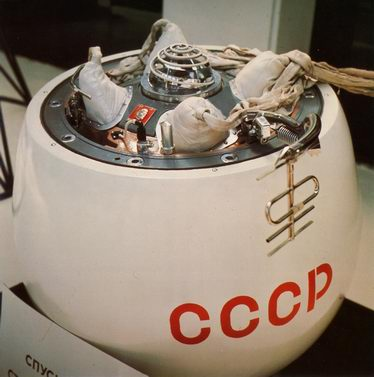
\includegraphics[scale=0.4]{./images/venera_7}
				\end{figure}
			\end{column}
		\end{columns}
	\end{frame}
	\subsection{Venera 8}
	\begin{frame}
		\begin{columns}
			\begin{column}{0.5\textwidth}
				\begin{itemize}
					\item 1972
					\item Sonde landete
					\item Auf Oberfläche waren 470$^\circ$C und 90bar
					\item Messung ergab ca. 1km Sichtweite
				\end{itemize}
			\end{column}
			\begin{column}{0.4\textwidth}
				\begin{figure}[ht]
					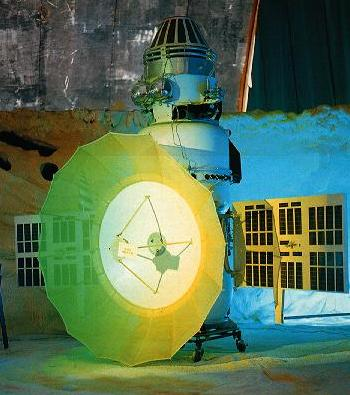
\includegraphics[scale=0.4]{./images/venera_8}
				\end{figure}
			\end{column}
		\end{columns}
	\end{frame}
	\section{Venera 9 \& 10}
	\subsection{Die Sonden}
	\begin{frame}
		\begin{itemize}
			\item 1975
			\item Sonden machten erstmals Fotos der Venus
			\item Arbeiteten beide ca. 1 Stunde
		\end{itemize}
	\end{frame}
	\subsection{Fotos von Venera 9}
	\begin{frame}
		\begin{figure}
			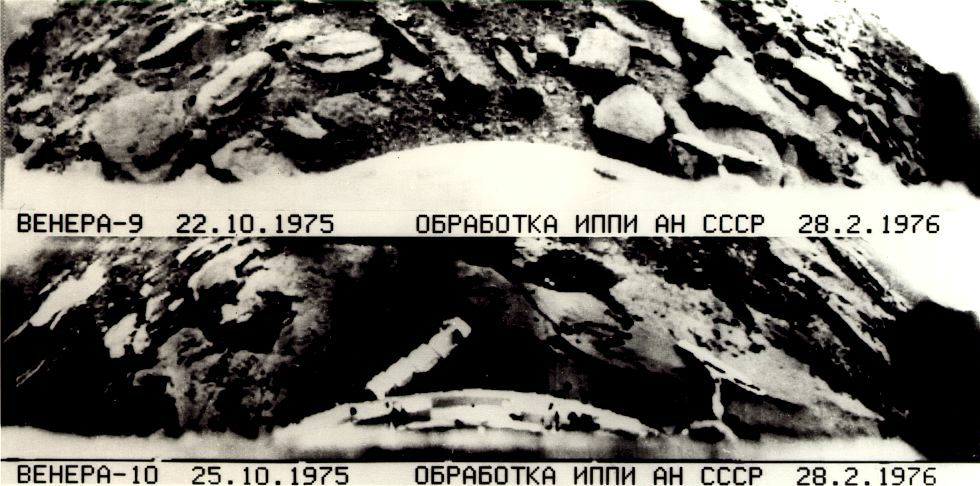
\includegraphics[scale=0.32]{./images/venera_9}
		\end{figure}
	\end{frame}
	\subsection{Fotos von Venera 10}
	\begin{frame}
		\begin{figure}
			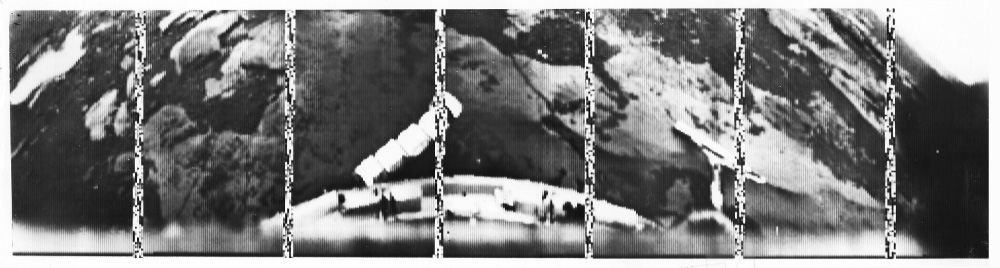
\includegraphics[scale=0.9]{./images/venera_10}
		\end{figure}
	\end{frame}
	\section{Venera 11, 12 \& 13}
	\begin{frame}
		\begin{itemize}
			\item 1978 und 1981
			\item Landeten alle
			\item Venera 13 machte Fotos
		\end{itemize}
	\end{frame}
	\begin{frame}
		\begin{figure}
			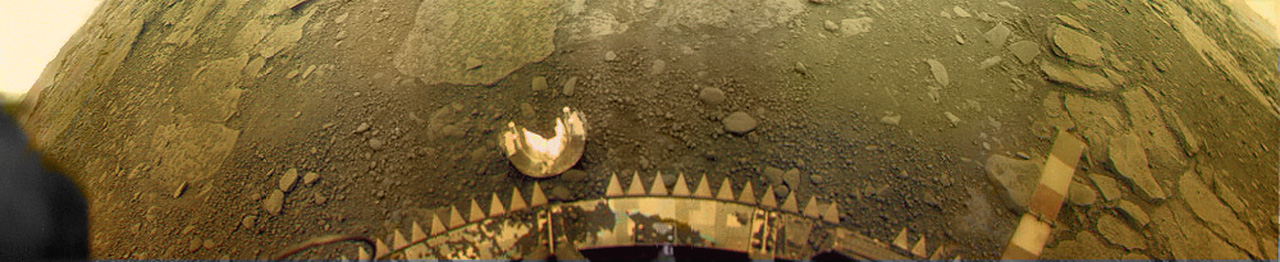
\includegraphics[scale=0.25]{./images/venera_13-1}
		\end{figure}
	\end{frame}
	\begin{frame}
		\begin{figure}
			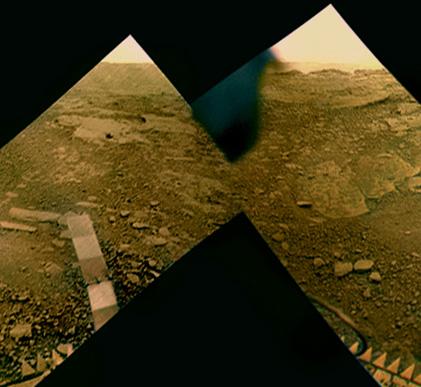
\includegraphics[scale=0.4]{./images/venera_13-2}
		\end{figure}
	\end{frame}
	\section{Venera 14}
	\begin{frame}
		\begin{itemize}
			\item 1981
			\item Letzte Landesonde auf der Venus
			\item Machte Fotos
			\item Bohrkopf fiel auf Kameraabdeckung
		\end{itemize}
	\end{frame}
	\begin{frame}
		\begin{figure}
			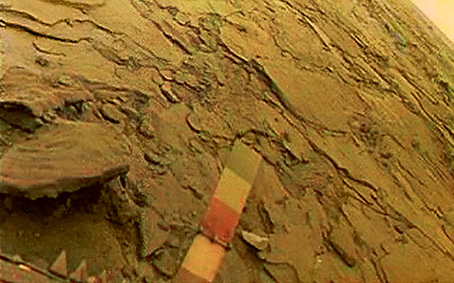
\includegraphics[scale=0.45]{./images/venera_14-1}
		\end{figure}
	\end{frame}
	\begin{frame}
		\begin{figure}
			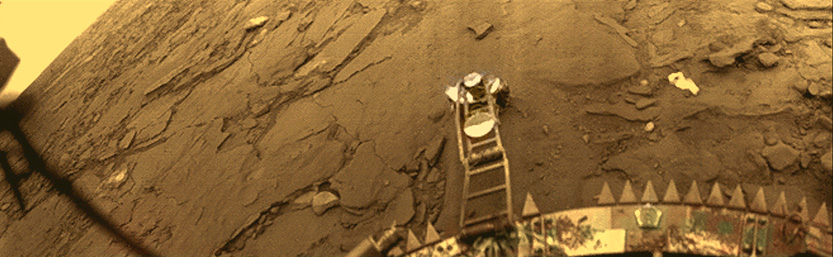
\includegraphics[scale=1.5]{./images/venera_14-2}
		\end{figure}
	\end{frame}
	\section{Venera 15 \& 16}
	\begin{frame}
		\begin{itemize}
			\item 1983
			\item Nur Orbiter
			\item Kartierung der Oberfläche
		\end{itemize}
	\end{frame}
	\begin{frame}
		\begin{figure}
			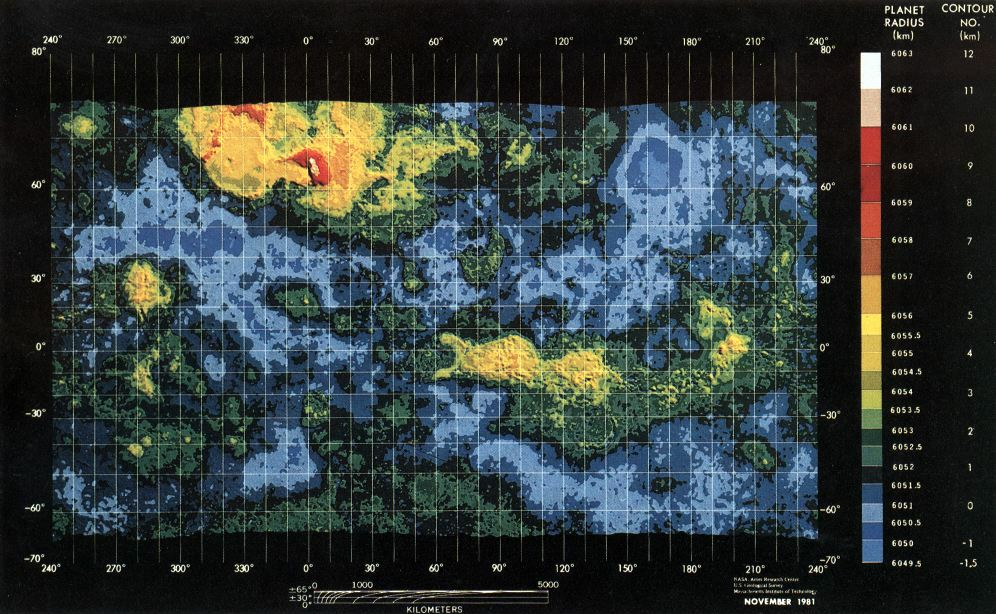
\includegraphics[scale=.3]{./images/schlaues_bild}
		\end{figure}
	\end{frame}
\end{document}